\documentclass[18pt]{beamer}
\usepackage[utf8]{inputenc}
% \usepackage{templates/mytemplate}
\usepackage{templates/beamerthemekit}
\usepackage{graphicx}
\usepackage{microtype}
\usepackage{listings}
\usepackage{color}
\usepackage{hyperref}
\usepackage{multicol}
\usepackage{siunitx}
\usepackage{physics}
\usepackage{booktabs}
\usepackage{longtable}
\usepackage{amssymb}

\lstset{ %
  backgroundcolor=\color{white},   % choose the background color; you must add \usepackage{color} or \usepackage{xcolor}; should come as last argument
  basicstyle=\tiny\ttfamily,
  xleftmargin=-10pt,
  breaklines=false,                 % sets automatic line breaking
  captionpos=b,                    % sets the caption-position to bottom
  % frame=single,	                   % adds a frame around the code
  keepspaces=true,                 % keeps spaces in text, useful for keeping indentation of code (possibly needs columns=flexible)
  language=C++,                 % the language of the code
  % morekeywords={*,...},            % if you want to add more keywords to the set
  tabsize=2,	                   % sets default tabsize to 2 spaces
  keywordstyle=\bfseries\color{kit-green70},
  commentstyle=\itshape\color{kit-blue70},
  identifierstyle=\color{black},
  stringstyle=\color{kit-orange100},  
}

\hypersetup{
    bookmarks=true,         % show bookmarks bar?
    colorlinks=true,       % false: boxed links; true: colored links
    linkcolor=red,          % color of internal links (change box color with linkbordercolor)
    citecolor=green,        % color of links to bibliography
    filecolor=magenta,      % color of file links
    urlcolor=kit-blue100           % color of external links
  }

\title{First look at Cosmic CDC Tracks and Ideas for Estimating the Finding Efficiency} 
\subtitle{F2F Tracking Meeting}
\author{\underline{Michael Eliachevitch}}
\date{19 September 2018}
\titleimage{transparent}
\institute{ETP - KIT}

\begin{document}

  \selectlanguage{english}

  \begin{frame}
  \titlepage
  \end{frame}

  \begin{frame}
    \frametitle{Introduction}
    \begin{itemize}
    \item First look cosmics data from Global Cosmic Run (GCR) 2017
    \item Reproduced of kinematic distributions, Data and MC
    \item Current tracking validation: Based on simulation and matching with MC Truth\\
      $\Rightarrow$ Is it possible to test the tracking on cosmics \emph{data} without MC truth?\\
      $\Rightarrow$ Compare with MC validation
    \end{itemize}
  \end{frame}

  \begin{frame}
    \frametitle{Used GCR Data and MC}
    \begin{itemize}
    \item first looked at GCR July run
      \begin{itemize}
      \item 6.4 Million data events of which I used 2.8 Million
      \item data used back-to-back TSF trigger condition
      \item trigger was at first not implemented 
      \end{itemize}
      $\Rightarrow$ total 2.8\,Million cosmic events with trigger selecting central tracks\\
    \item also produced 50\,Million cosmic MC events with GCR setup
      \begin{itemize}
      \item same as official MC group: large ``accept box'' of 8\,m $\times$ 8\,m $\times$ 8\,m 
      \item no trigger in simulation, do kinematic cuts on central region ($d_0, z_0$)\\
        $\Rightarrow$  $\sim$10 times less statistics than in data remain
      \end{itemize}
    \end{itemize}

    \begin{block}{Links to information on data and MC production}
      \begin{itemize}
      \item Data: \footnotesize{\url{https://confluence.desy.de/display/BI/Data+Production+Global+Cosmics+Run+Data\#DataProductionGlobalCosmicsRunData-Runinfo}}
      \item MC: \footnotesize{\url{https://confluence.desy.de/display/BI/Data+Production+Global+Cosmics+Run+MC}}
      \end{itemize}
    \end{block}
  \end{frame}

  \begin{frame}
    \frametitle{Kinematic Distributions: Data and MC}
    \begin{itemize}
    \item left data (includes trigger), right MC (without trigger)
    \item use (preliminary) cuts for selection of central tracks (red lines)
    % \item B-Field mapper not in simulation
    \end{itemize}
    \begin{center}
      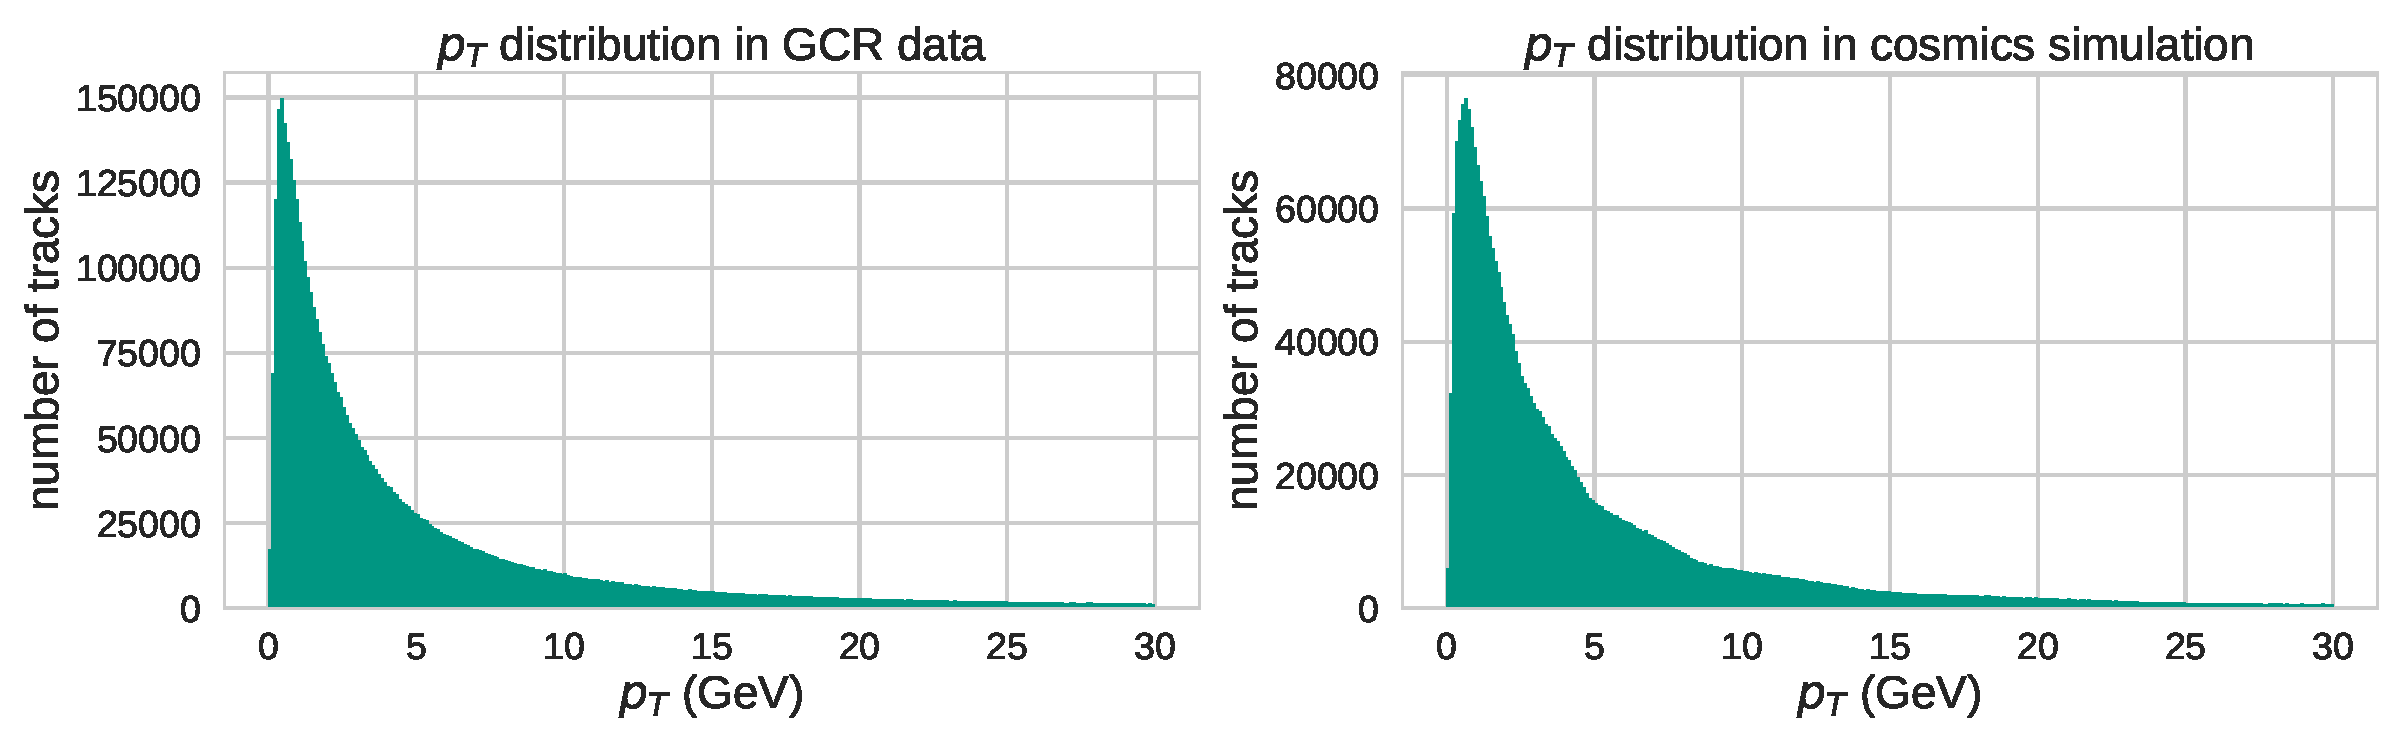
\includegraphics[width=0.8\textwidth]{figures/distributions/gcr_pt_distribution_uncut.pdf}\\
      \includegraphics[width=0.8\textwidth]{figures/distributions/gcr_omega_distribution_uncut.pdf}
    \end{center}
    \begin{itemize}
    \item $p_T$ distributions seem similar, but more events with $\omega = 0$
    \end{itemize}
  \end{frame}

  \begin{frame}
    \begin{center}
      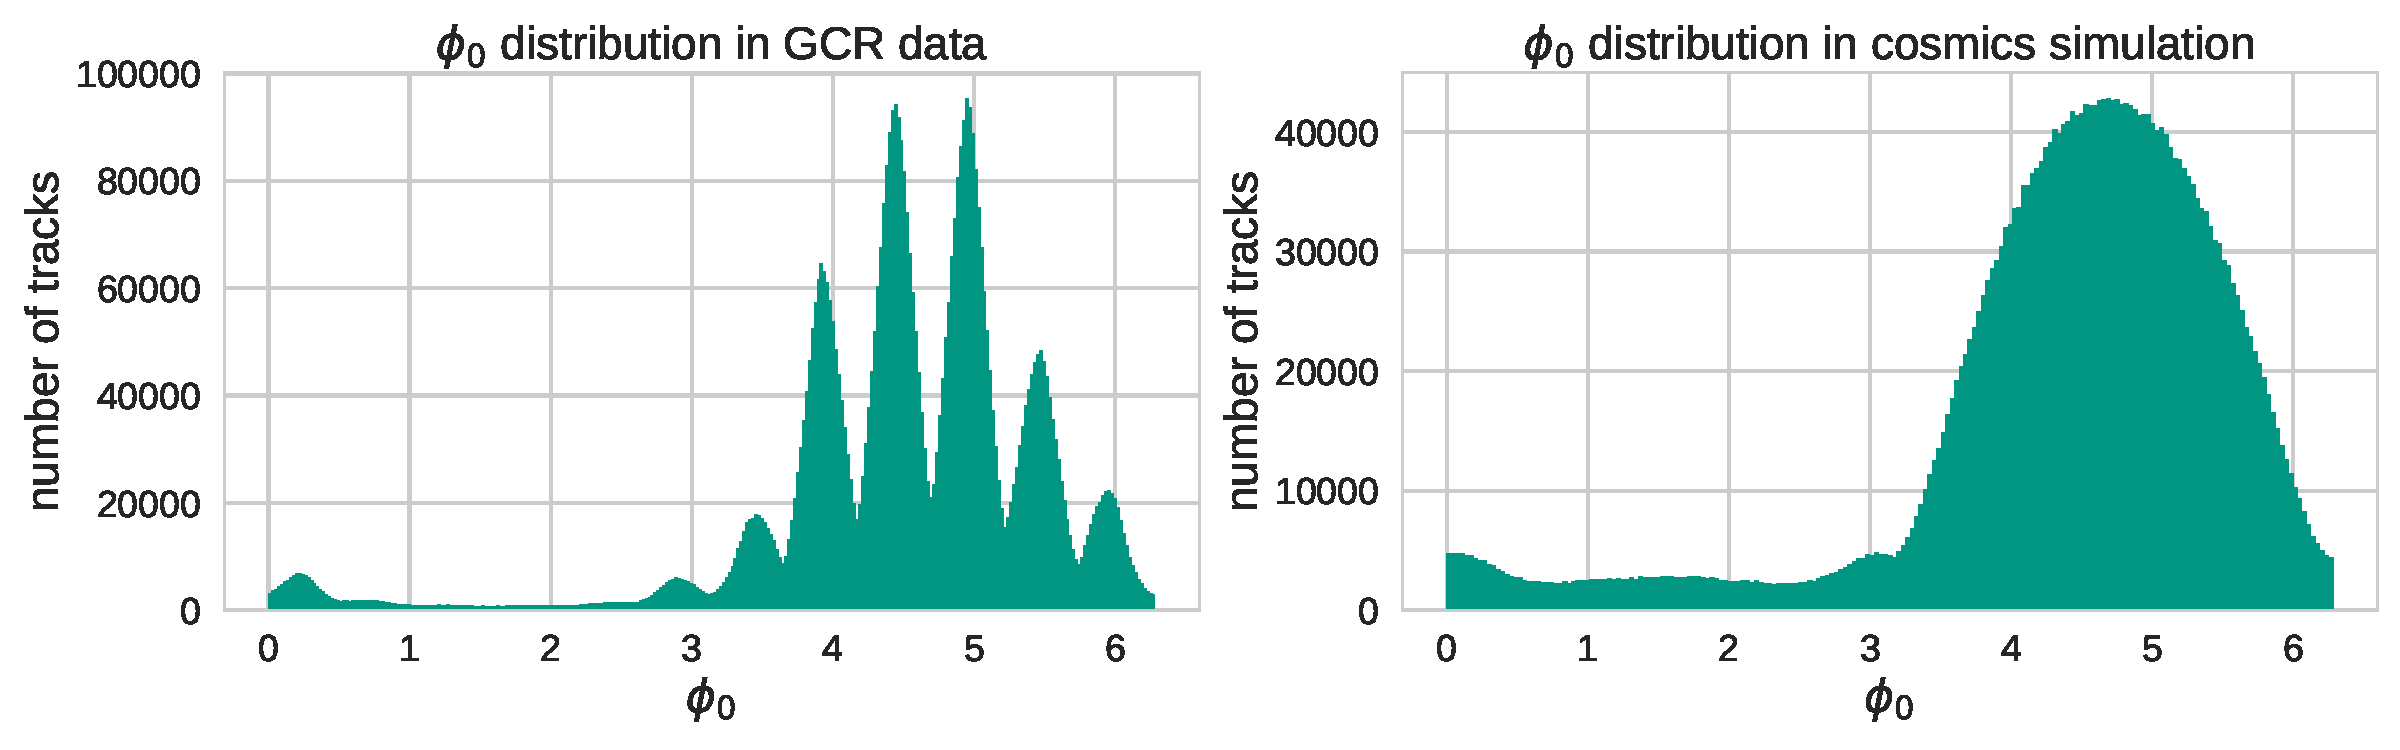
\includegraphics[width=0.8\textwidth]{figures/distributions/gcr_phi0_distribution_uncut.pdf}\\
      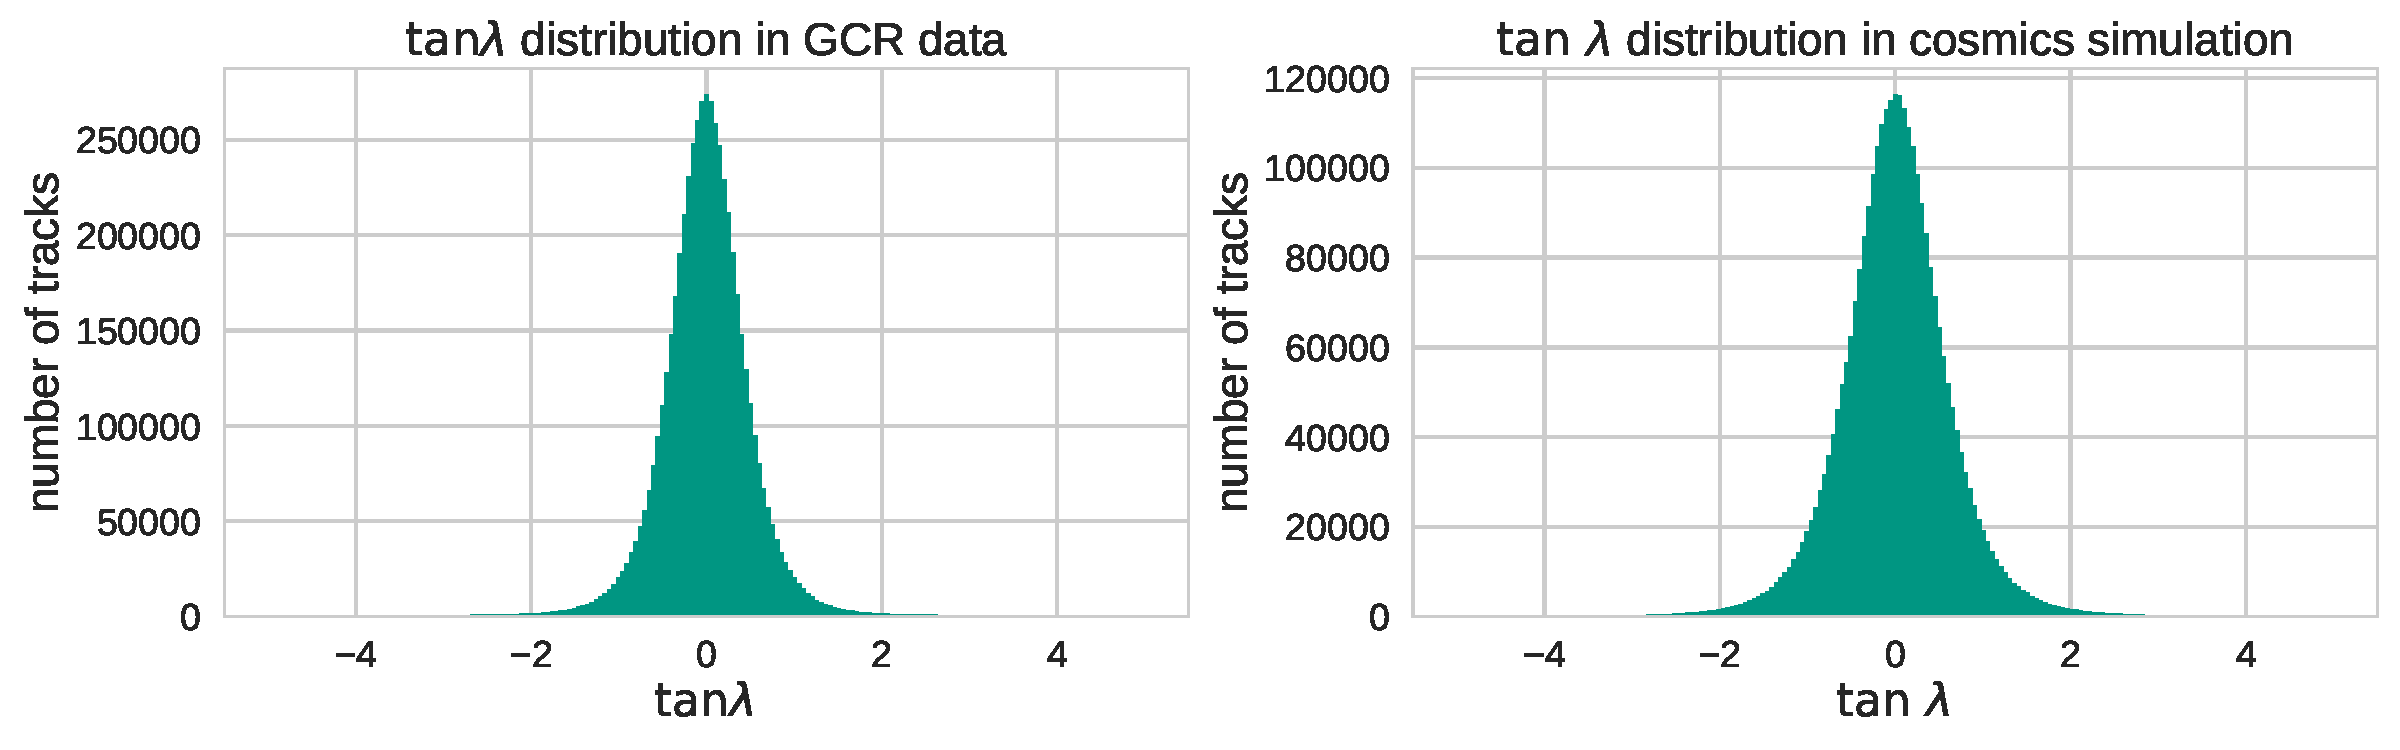
\includegraphics[width=0.8\textwidth]{figures/distributions/gcr_tan_lambda_distribution_uncut.pdf}
    \end{center}

    \begin{itemize}
    \item modulation in $\phi_0$ due to varying trigger efficiencies
    \end{itemize}
  \end{frame}

  \begin{frame}
    \begin{center}
      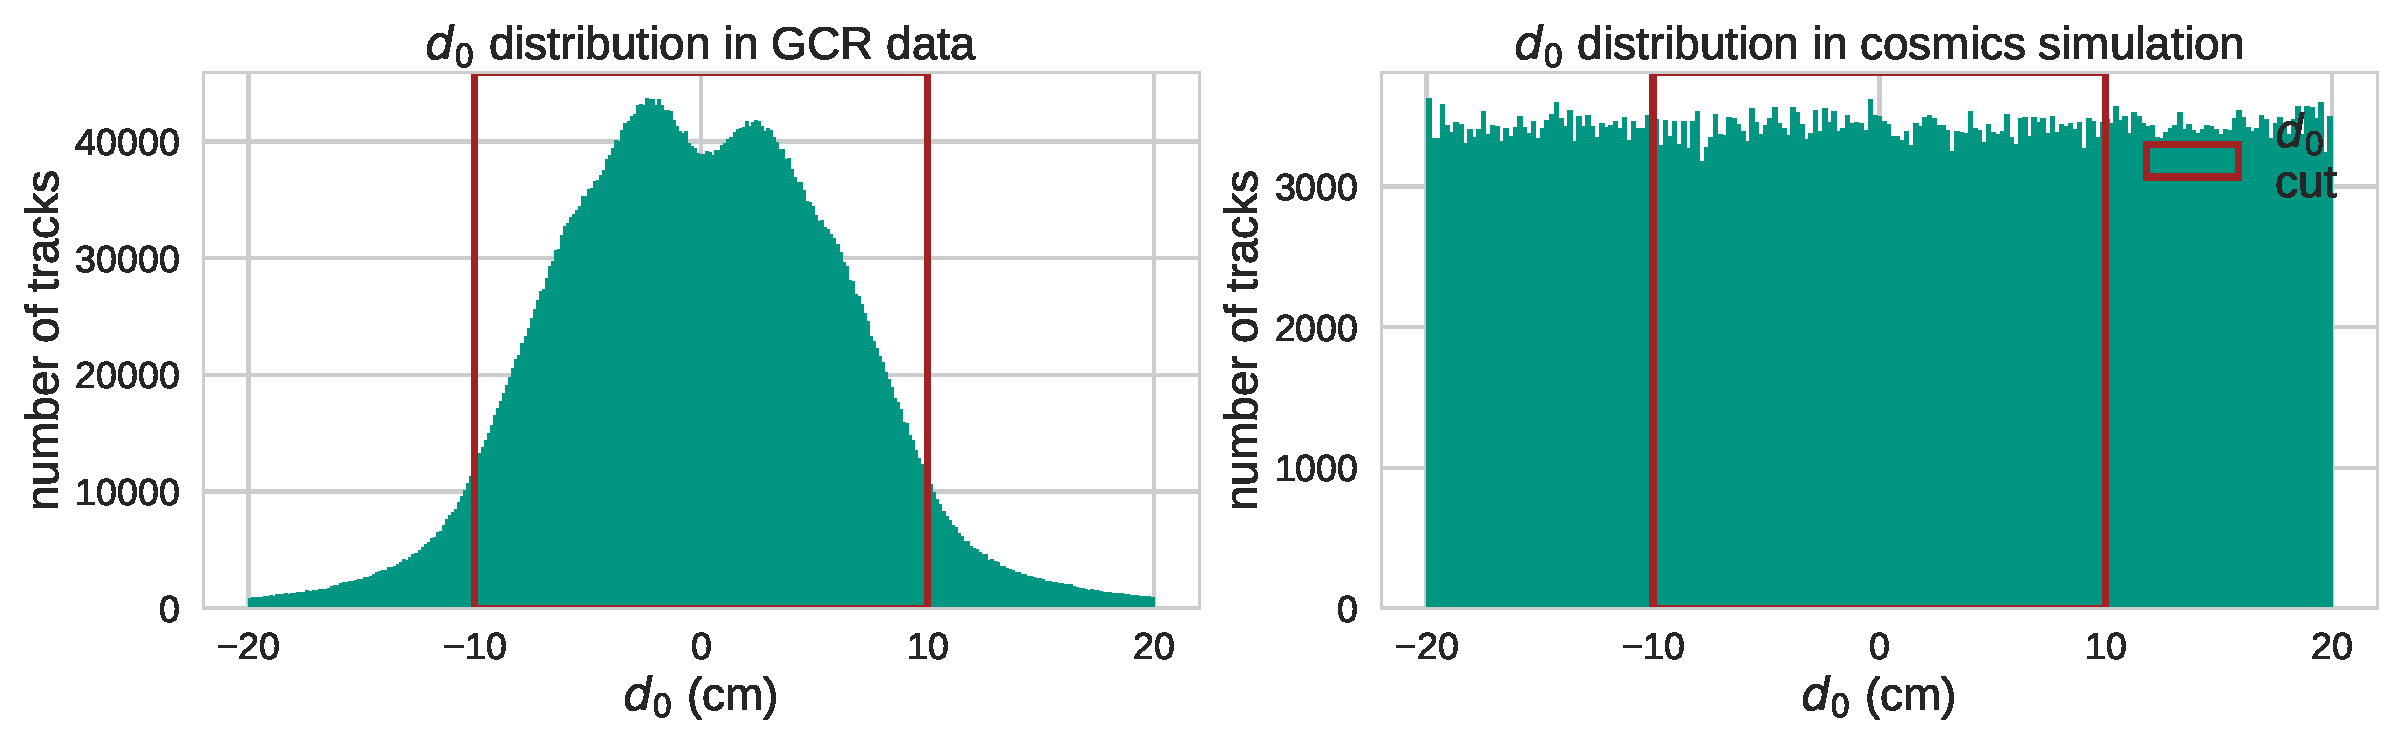
\includegraphics[width=0.8\textwidth]{figures/distributions/gcr_d0_distribution_uncut.pdf}\\
      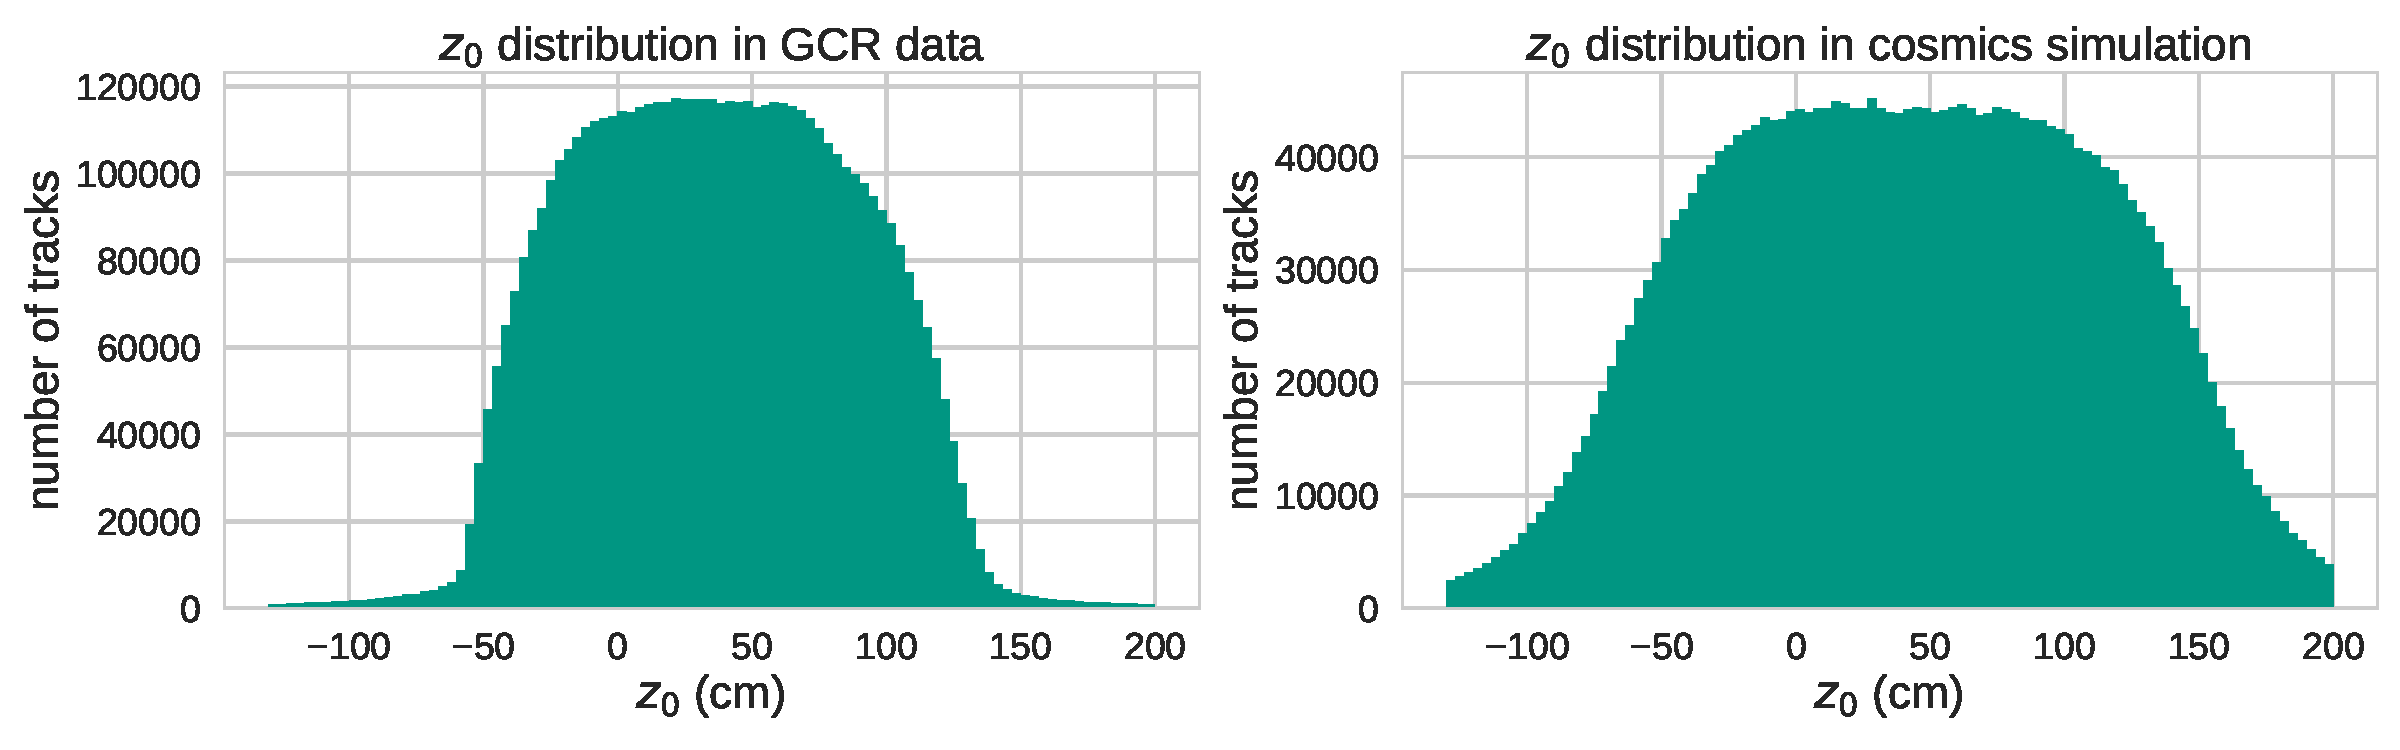
\includegraphics[width=0.8\textwidth]{figures/distributions/gcr_z0_distribution_uncut.pdf}
    \end{center}
    \begin{itemize}
    \item distribution in MC due to lack of trigger much wider, use cuts on central region
    \end{itemize}
  \end{frame}

  \begin{frame}
    \frametitle{Idea: Cosmics-based Estimation of Finding Efficiency}
    \begin{itemize}
    \item Typical event: Single muon track, usually no secondaries
    \item tracks passing through the central SVD volume are split
    \item reconstructed as two \texttt{NonMergedRecoTracks},
      which are then merged to \texttt{RecoTracks}
    \item get estimate of finding efficiency from events where two tracks expected, but only one found (finding fails)
    \end{itemize}
    \pause
    \begin{block}{}
      \begin{equation*}
        \label{eq:cosmic_eff}
        \text{Finding efficiency} = \frac{N_\mathrm{2\ tracks\ found}}{N_\mathrm{2\ tracks\ expected}}
        = 1 - \frac{N_\mathrm{1\ track\ found}}{N_\mathrm{2\ tracks\ expected}}
      \end{equation*}             %
    \end{block}
    where $N_\mathrm{1\ track\ found}, N_\mathrm{2\ tracks\ found}, \in N_\mathrm{2\ tracks\ expected}$, so that $N_\mathrm{1\ track\ found} + N_\mathrm{2\ tracks\ found} = N_\mathrm{2\ tracks\ expected}$.
    \centering
    % \includegraphics[width=0.3\textwidth]{figures/b2display_example_1trackevt_cut.png}
  \end{frame}

  \begin{frame}
    \frametitle{Selection of Expected Events with two Tracks in MC and Data}
    \begin{itemize}
    \item need to select events where 2 (findable) \texttt{RecoTrack}s are expected
    \item this needs to be independent of actual number of tracks in event
    \item<2-> use cuts:
      \begin{itemize}
      \item kinematic cuts on $d_0$, $z_0$, \ldots to select events where tracks went through SVD volume
      \item cuts on hit content, e.g. minimum amount of CDC hits, hit positions?
      \end{itemize}
    \item<3-> the choice of cuts and the assessment of the selection quality require MC truth
    \item<3-> \textcolor{kit-red100}{Problem:} Tracks not split in MC, only one \texttt{MCRecoTrack} per particle
    \end{itemize}
  \end{frame}

  \begin{frame}
    \frametitle{Split MC Tracks on $\Delta t$ between Hits}
    \begin{itemize}
    \item split \texttt{MCRecoTrack} when time between subsequent \texttt{CDCSimHit}s is larger than chosen $\Delta t$
    \item add new parameter \texttt{SplitAfterDeltaT} to \texttt{TrackFinderMCTruthRecoTracksModule}
    \item \href{https://stash.desy.de/projects/B2/repos/software/pull-requests/737}{pull request} has already been merged
    \item choose high enough $\Delta t$ to only split on passing through SVD volume
    \item<4> method not yet used, still a \textcolor{kit-red100}{WIP}
    \end{itemize}
    \begin{center}
      \includegraphics<1>[width=0.45\textwidth]{figures/delta_t/delta_t_log.pdf}
      \includegraphics<1>[width=0.45\textwidth]{figures/delta_t/delta_t_max_log.pdf}
      \includegraphics<2>[width=0.45\textwidth]{figures/delta_t/delta_t_linear.pdf}
      \includegraphics<2>[width=0.45\textwidth]{figures/delta_t/delta_t_max_linear.pdf}
      \includegraphics<3->[width=0.45\textwidth]{figures/delta_t/delta_t_linear_annotated.pdf}
      \includegraphics<3->[width=0.45\textwidth]{figures/delta_t/delta_t_max_linear_annotated.pdf}
    \end{center}
  \end{frame}

  \begin{frame}
    \frametitle{Naive, preliminary Cuts for testing (not from MC)}
    \begin{itemize}
    \item MC truth for cut opimization and testing has just become available, not used yet
    \item before that, I still wanted to test the method for efficency estimation
    \item previously shown kinematic cuts to select central events:\\
      $\abs{d_0} < \SI{10}{\cm}$, $\SI{-50}{\cm} < z_0 < \SI{125}{\cm}$,  $\abs{\tan \lambda} < 1$
    \item chose preliminary, ``intuitive'' cuts on hit content, based on distributions of hit content with 1/2 \emph{found} tracks
    \end{itemize}
    \pause
    \begin{block}{Naive selection of candidate events for efficiency estimation}
      cuts on hit content for one track events only:
      \begin{itemize}
      \item \# hits in events $>$ 85
      \item \# missing CDC hits $>$ 45\%
      \item \textcolor{red}{Uncontrolled systematics, biased, just for testing!}
      \end{itemize}
    \end{block}
  \end{frame}

  \begin{frame}
    \frametitle{False Finding Fail Candidate (``Background'')}
    \begin{itemize}
    \item many tracks leave acceptance after passing through SVD volume
    \item this event leaves enough hits in the second hough to pass through my naive cuts on hit content $\rightarrow$ need for more sophisticated methods
    \end{itemize}
    \begin{center}
      \includegraphics[width=0.7\textwidth]{figures/b2display_example_bkgevt.png}
    \end{center}
  \end{frame}

  \begin{frame}
    \frametitle{WIP: Future Selection of Candidate Events}
    \begin{itemize}
    \item choose cuts and analyze systematics based on MC Truth (from \texttt{SplitAfterDeltaT} and further constraints)
    \item candidate events with two expected tracks chosen without knowledge of how many tracks were found
    \item more sophisticated selection methods, use hit positions
      \begin{itemize}
      \item e.g. select tracks where $\abs{\sum_i z_i} < \Delta z$
      \end{itemize}
    \end{itemize}
  \end{frame}

  \begin{frame}
    \frametitle{Distributions of the number of CDC Hits}
    \includegraphics[width=0.9\textwidth]{figures/hit_content_1dhistograms.pdf}
  \end{frame}

  \begin{frame}
    \frametitle{Total CDC Hits vs. Matched CDC Hits}
    \large In MC:\\
    \begin{center}
      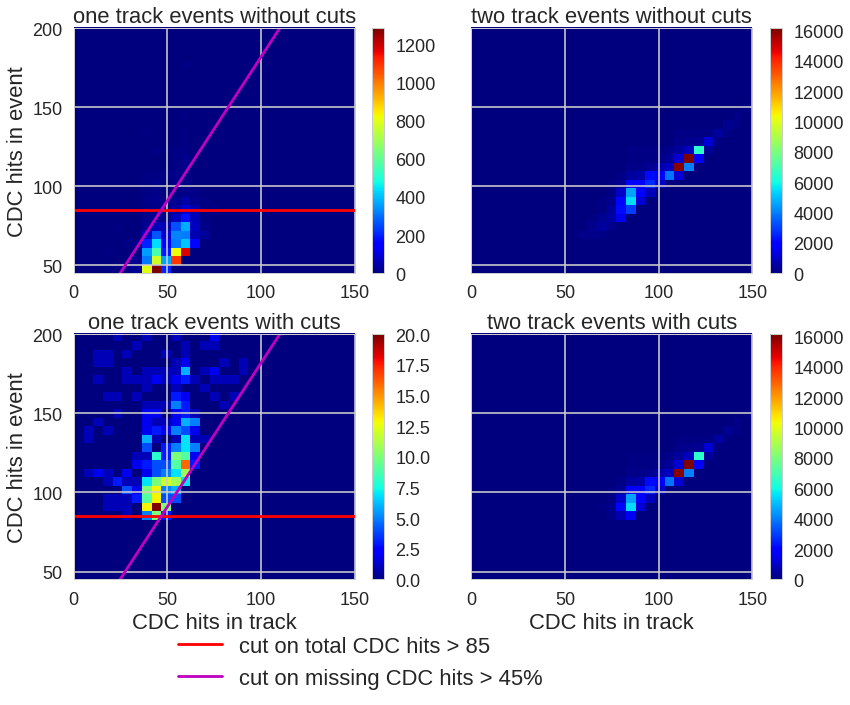
\includegraphics[width=0.73\textwidth]{figures/hitcontent_2dhist_MC.png}
    \end{center}
  \end{frame}

  \begin{frame}
    \frametitle{Total CDC Hits vs. Matched CDC Hits}
    \large In Data:\\
    \begin{center}
      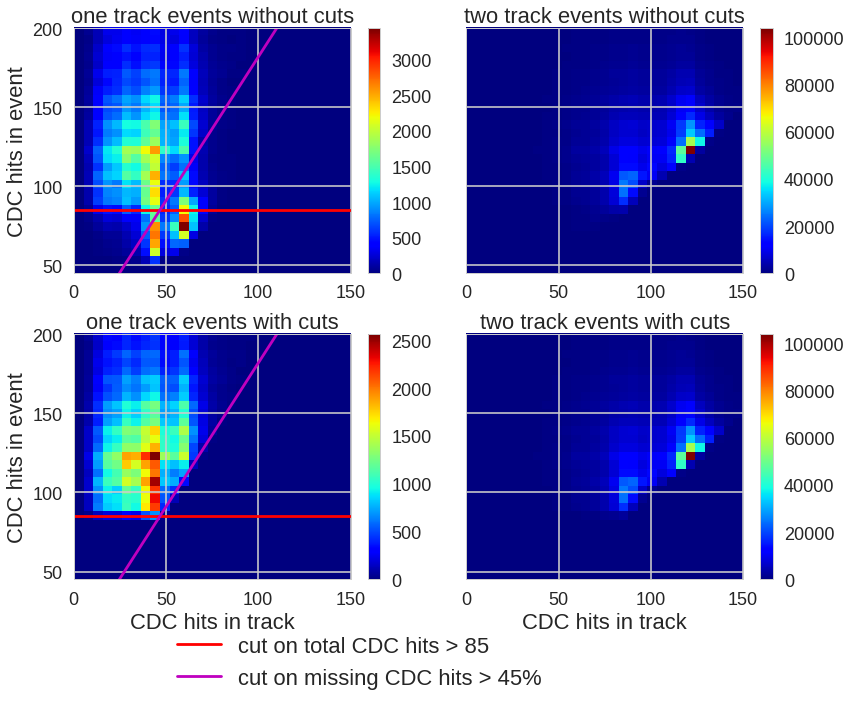
\includegraphics[width=0.73\textwidth]{figures/hitcontent_2dhist_data.png}
    \end{center}
  \end{frame}

  \begin{frame}
    \frametitle{``Efficiency'' Profiles with Naive Cuts}
    \begin{alertblock}{Reminder}
      Results for $N_2 / (N_1 + N_2)$ with naive cuts. Not neccessarily related to actuall efficiency yet!
    \end{alertblock}
    \begin{center}
      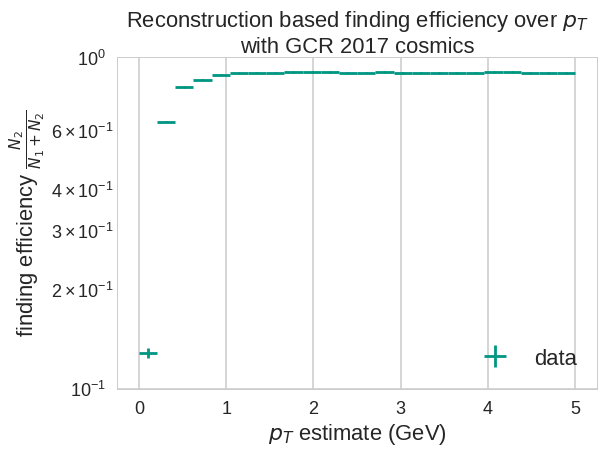
\includegraphics[width=0.49\textwidth]{figures/findeff_pt_data.png}
      \includegraphics[width=0.49\textwidth]{figures/findeff_d0_data.png}
    \end{center}
  \end{frame}
  \begin{frame}
    \begin{center}
      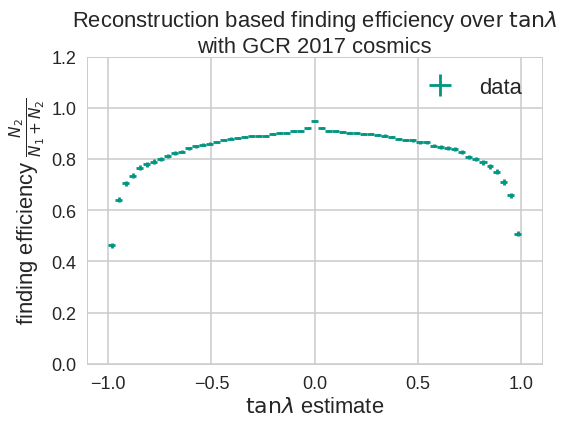
\includegraphics[width=0.49\textwidth]{figures/findeff_tan_lambda_data.png}
      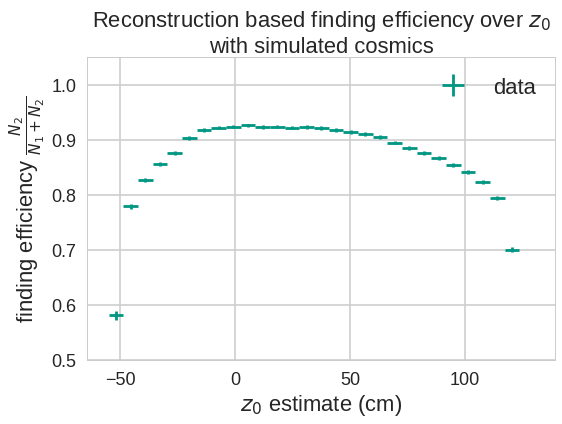
\includegraphics[width=0.49\textwidth]{figures/findeff_z0_data.png}\\
      \includegraphics[width=0.49\textwidth]{figures/findeff_phi0_data.png}
    \end{center}
  \end{frame}
  
  \begin{frame}\label{lastbeforebackup}
    \frametitle{Outlook / TODO}
    \begin{itemize}
    \item get MC information on number of Reco Tracks with \texttt{SplitAfterDeltaT} and use it to test our methods
    \item with MC information, develop more sophisticated selection of events with two findable tracks
    \item finding efficiency profiles should be the same on MC and data
    \item see if efficiency profiles are similar to those of MC Matcher Truth
    \end{itemize}
  \end{frame}

  \backupbegin

  \begin{frame}
    \begin{center}
      \huge Backup
    \end{center}
  \end{frame}

    \begin{frame}
    \begin{center}
      \frametitle{Example Finding Fail Event}
      \includegraphics[width=0.7\textwidth]{figures/b2display_example_1trackevt.png}
    \end{center}
  \end{frame}

    \begin{frame}[allowframebreaks]
    \frametitle{Kinematic Distributions with Kinematic Cuts}
    \begin{center}
      \includegraphics[width=0.65\textwidth]{figures/distributions/gcr_pt_distribution_cut.pdf}\\
      % 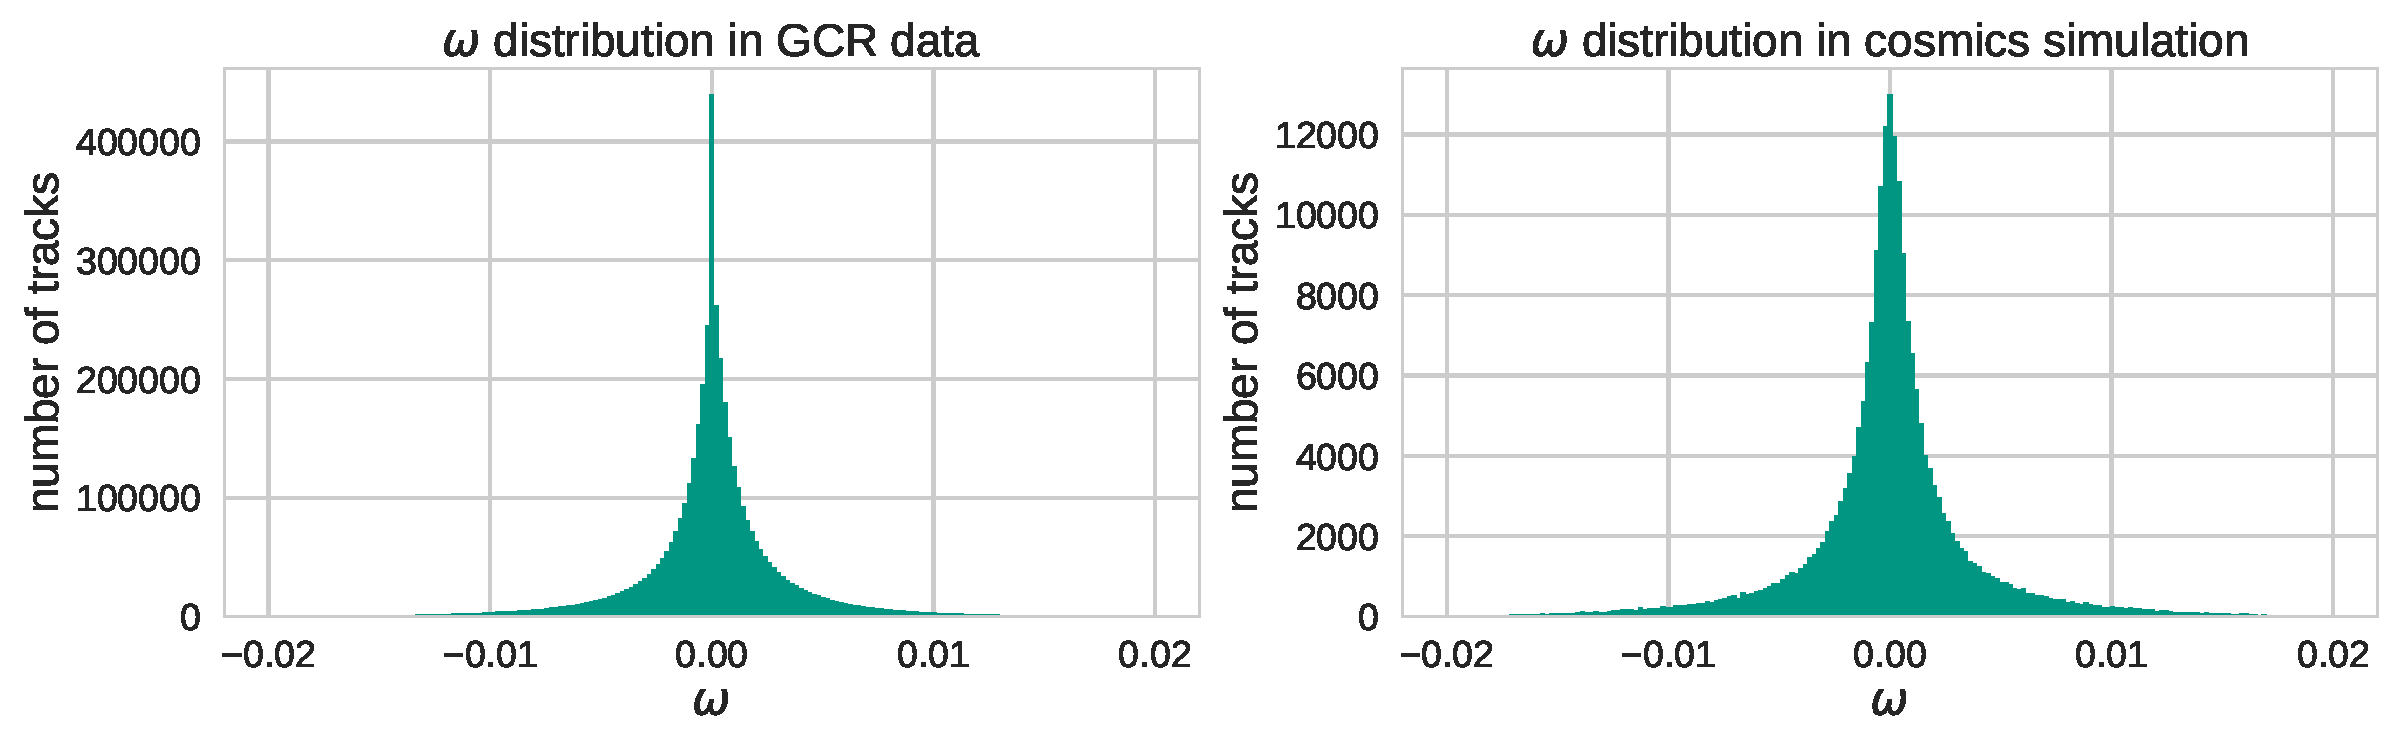
\includegraphics[width=0.65\textwidth]{figures/distributions/gcr_omega_distribution_cut.pdf}\\
      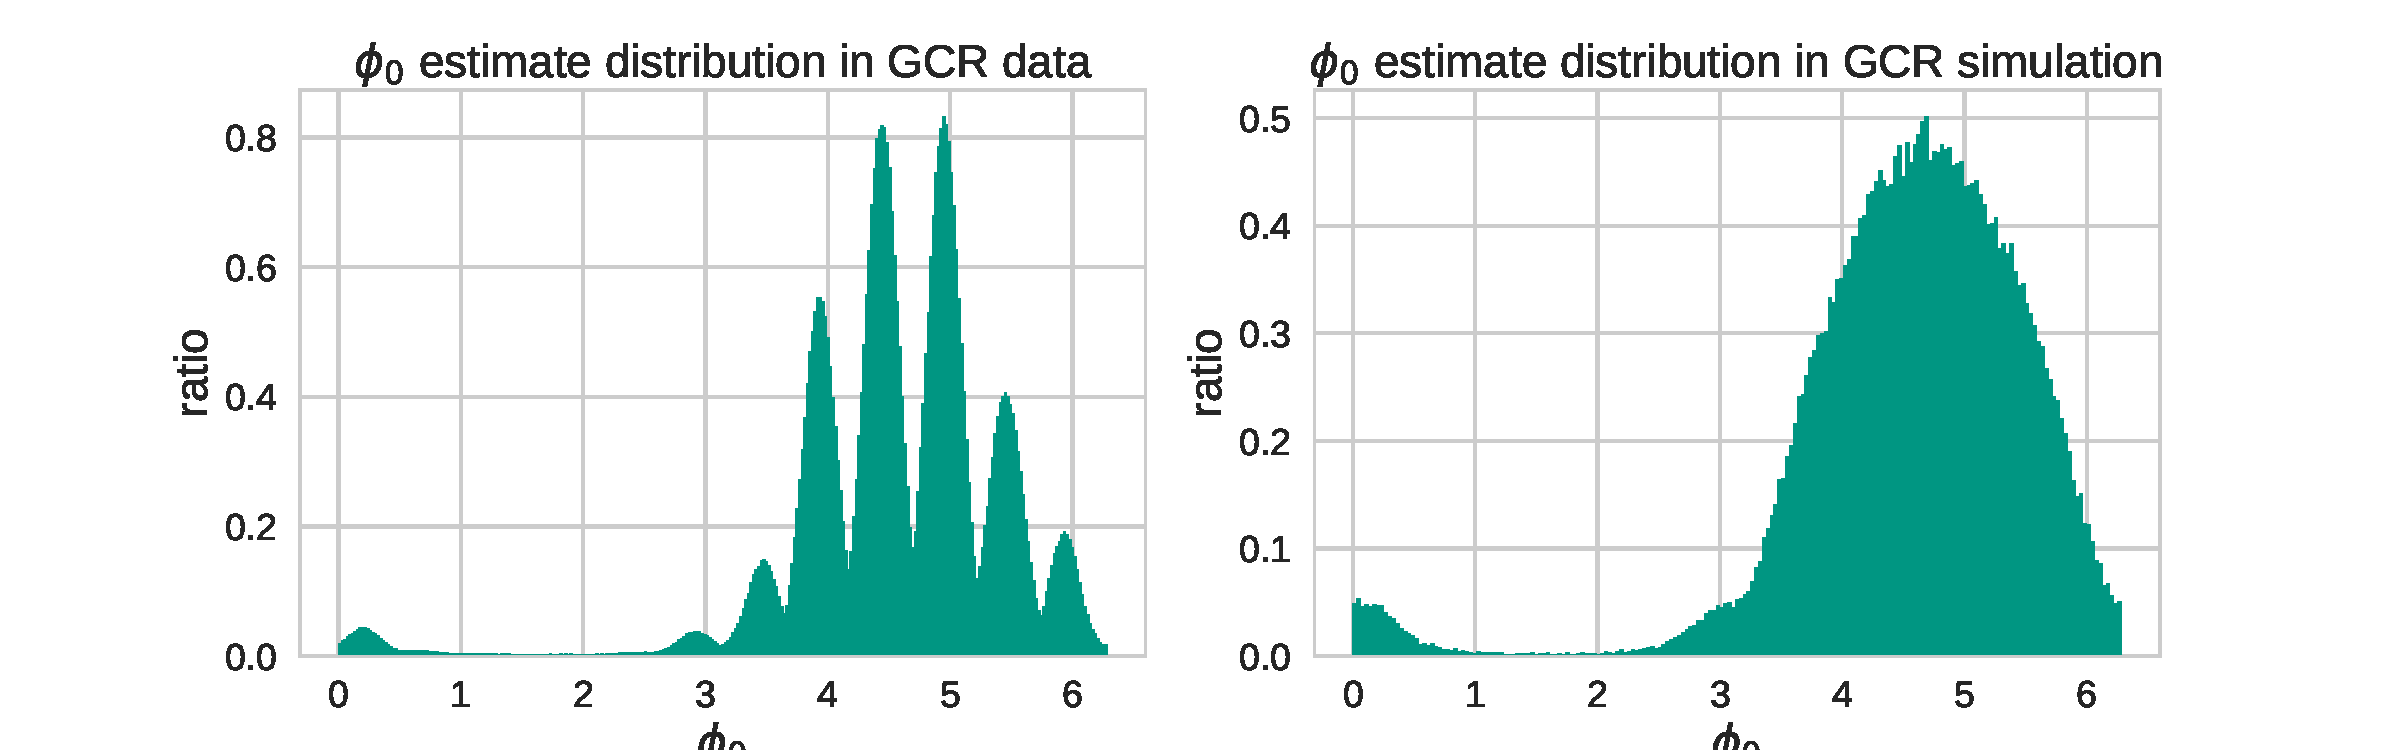
\includegraphics[width=0.65\textwidth]{figures/distributions/gcr_phi0_distribution_cut.pdf}\\
      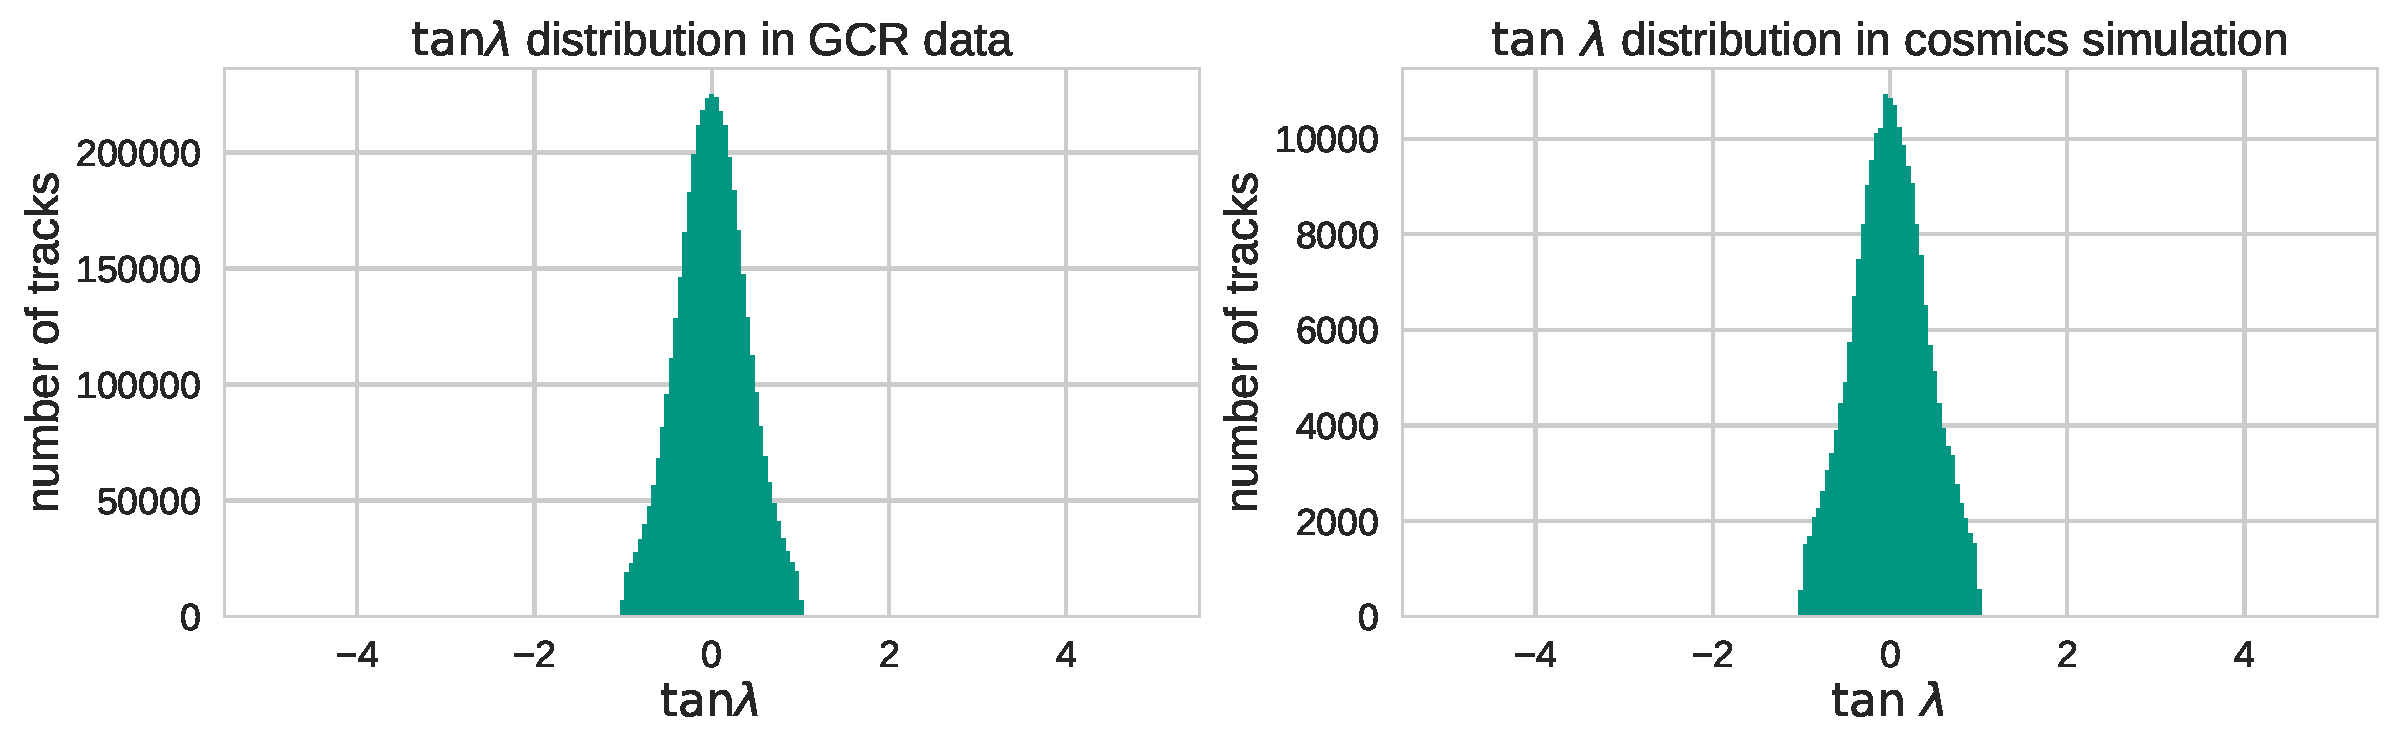
\includegraphics[width=0.65\textwidth]{figures/distributions/gcr_tan_lambda_distribution_cut.pdf}\\
      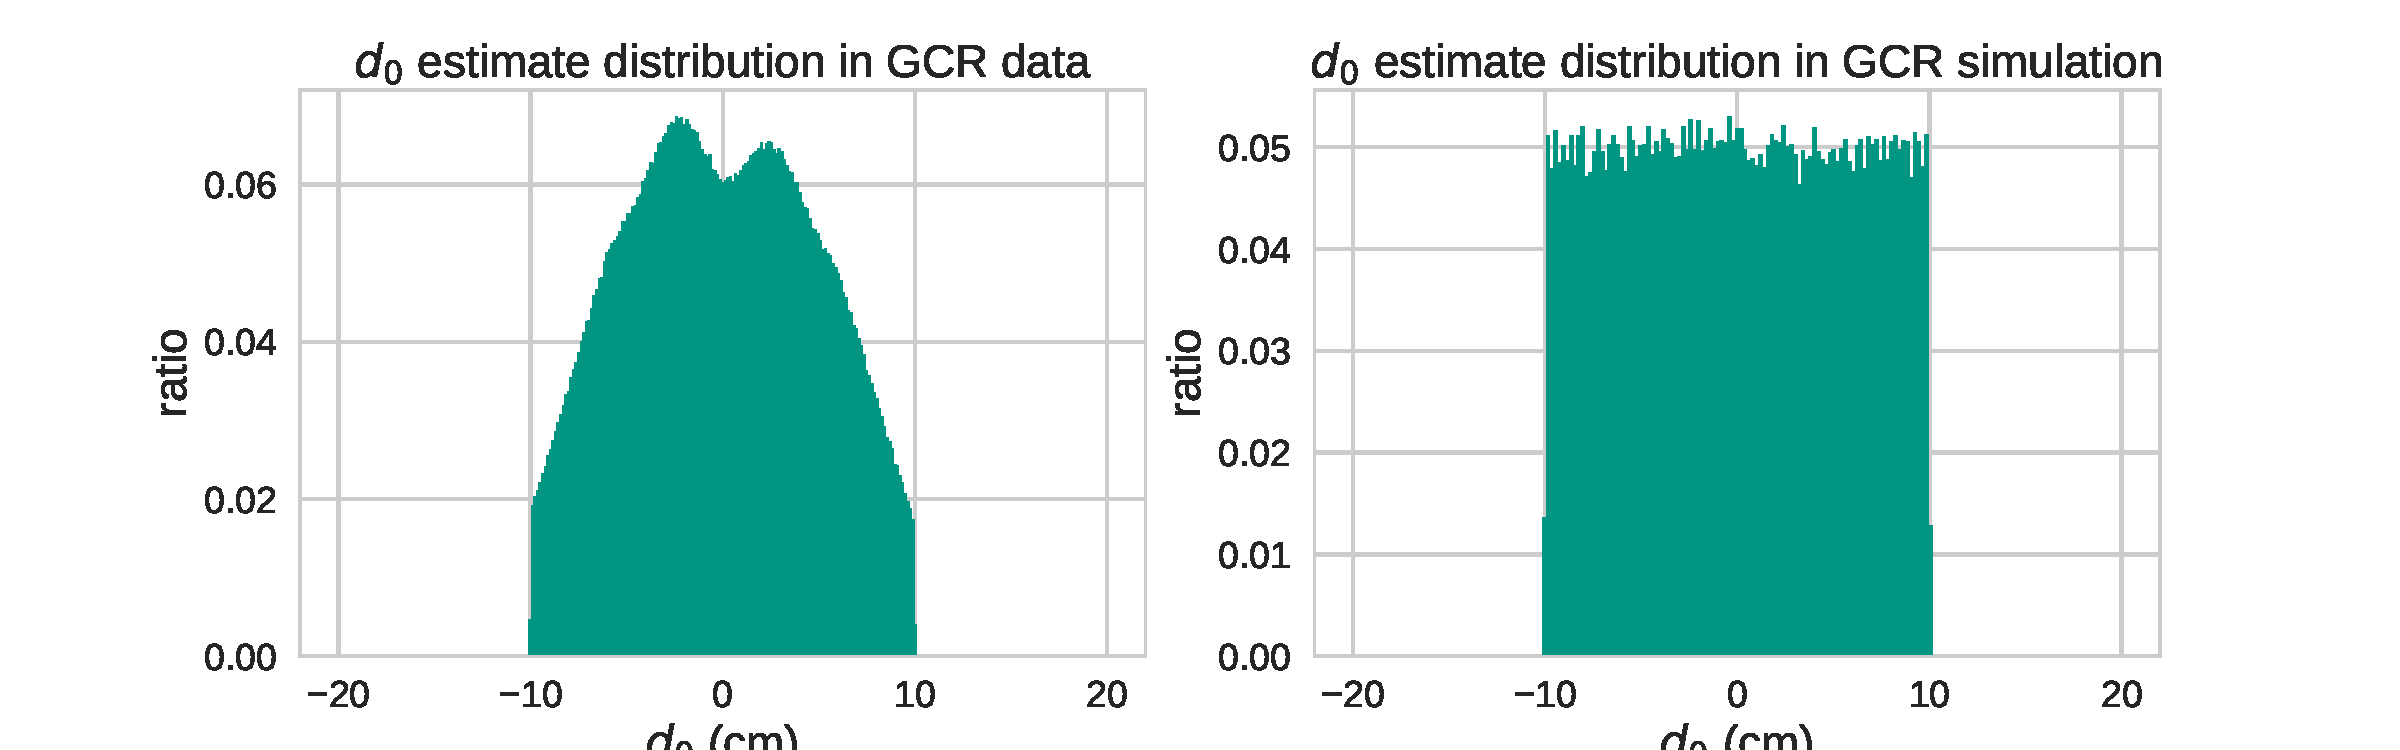
\includegraphics[width=0.65\textwidth]{figures/distributions/gcr_d0_distribution_cut.pdf}\\
      \includegraphics[width=0.65\textwidth]{figures/distributions/gcr_z0_distribution_cut.pdf}

    \end{center}
  \end{frame}

  \begin{frame}[fragile]
    \frametitle{Code for Splitting Tracks in MC Track Finder}
    \begin{lstlisting}[language=C++]
std::vector< std::vector<TimeHitIDDetector> > hitsWithTimeAndDetectorInformationVectors;

if (m_splitAfterDeltaT < 0.0) { // no splitting, vector will only contain a single hitInformation vector
  hitsWithTimeAndDetectorInformationVectors.push_back(hitsWithTimeAndDetectorInformation);
} else { // split on delta t

  std::vector<TimeHitIDDetector>::size_type splitFromIdx = 0; // whenever splitting subtrack, start slice from this index
  for (std::vector<TimeHitIDDetector>::size_type i = 1; i != hitsWithTimeAndDetectorInformation.size(); i++) {

    double delta_t = (std::get<0>(hitsWithTimeAndDetectorInformation[i])
                      - std::get<0>(hitsWithTimeAndDetectorInformation[i - 1]));

    if (delta_t > m_splitAfterDeltaT) {
      // push slice of `hitsWithTimeAndDetectorInformation' between splitFromidx  and previous index
      hitsWithTimeAndDetectorInformationVectors
      .emplace_back(hitsWithTimeAndDetectorInformation.begin() + splitFromIdx,
                    hitsWithTimeAndDetectorInformation.begin() + i);
      splitFromIdx = i;
    }
  }
  // add subtrack after last splitting to list of tracks
  hitsWithTimeAndDetectorInformationVectors
  .emplace_back(hitsWithTimeAndDetectorInformation.begin() + splitFromIdx,
                hitsWithTimeAndDetectorInformation.end());
}
    \end{lstlisting}
  \end{frame}

  \begin{frame}[allowframebreaks]
    \frametitle{Track Numbers with different Cuts}
    \begin{itemize}
    \item with no cuts:\\
      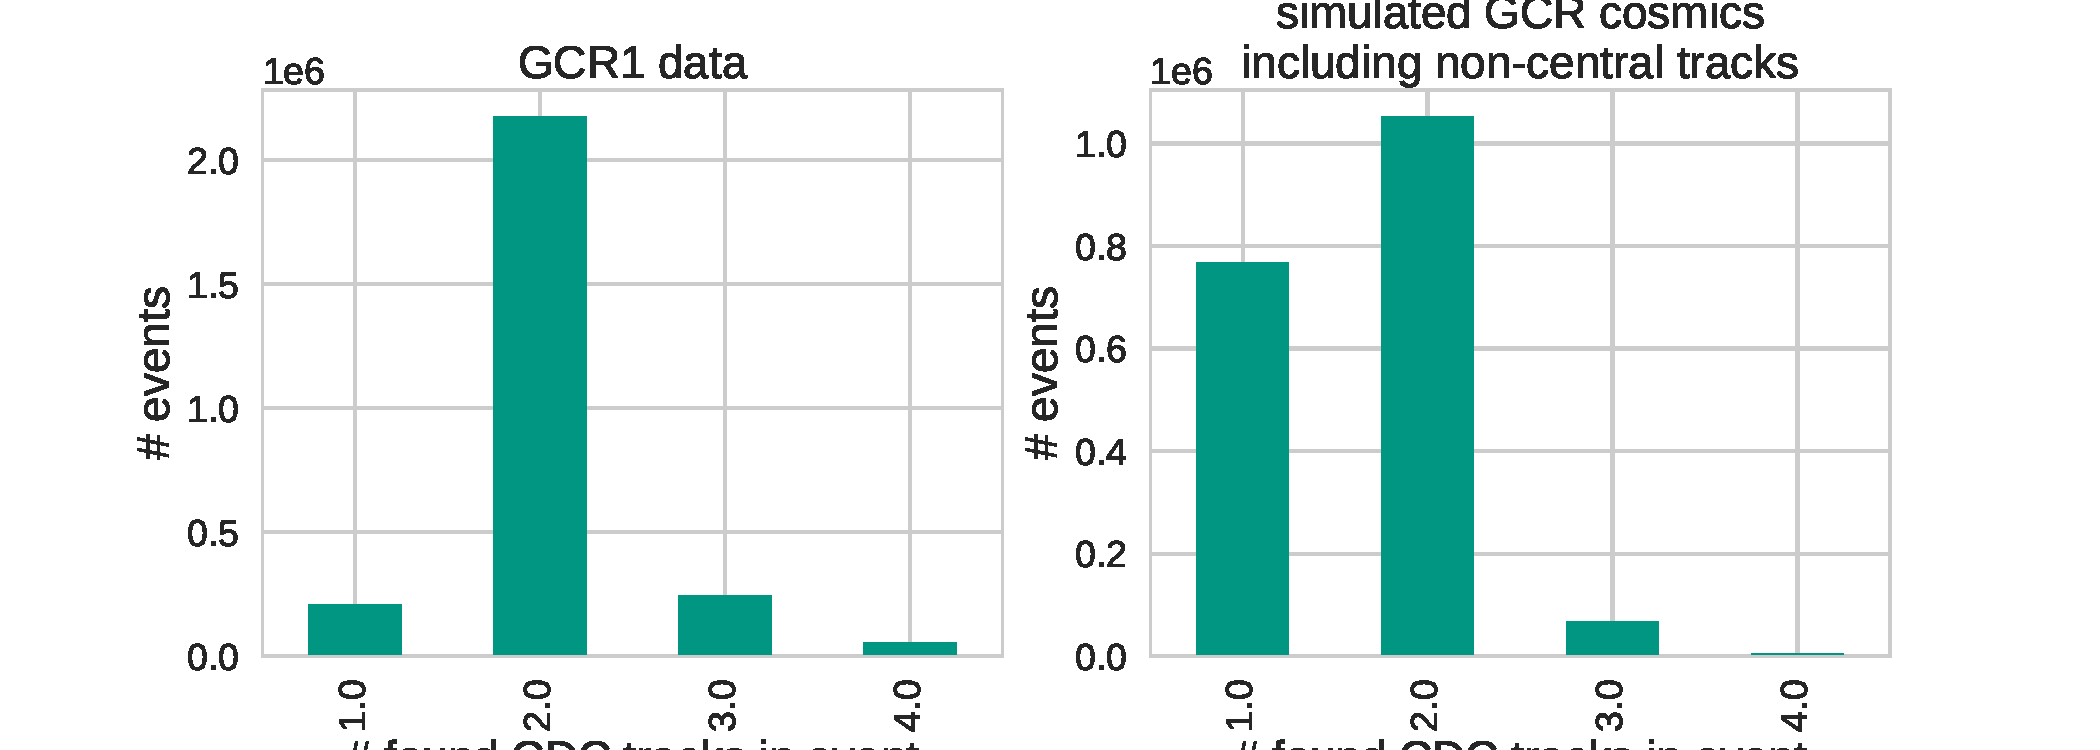
\includegraphics[width=0.7\textwidth]{figures/nfound_tracks_nocuts.pdf}
    \item with kinematic cuts:
      \includegraphics[width=0.7\textwidth]{figures/nfound_tracks_kincuts.pdf}\\      
    \item with cuts on hit content:\\
      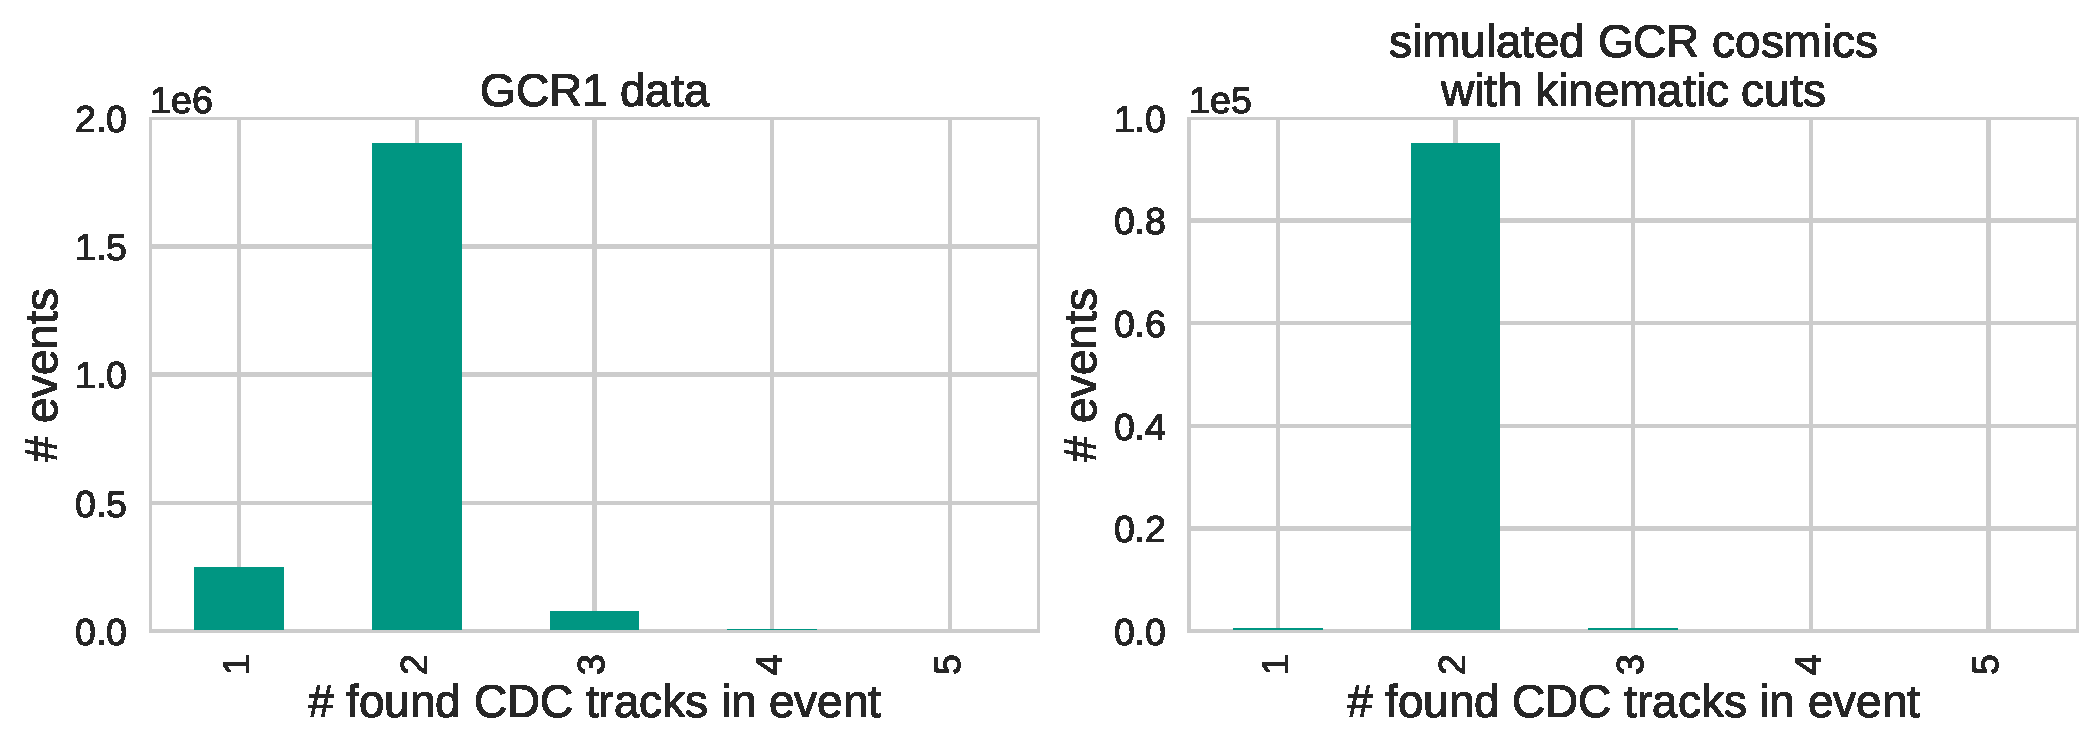
\includegraphics[width=0.7\textwidth]{figures/nfound_tracks_allcuts.pdf}
    \end{itemize}
  \end{frame}

  \begin{frame}[allowframebreaks]
    \frametitle{Runinfo for GCR data used by me}
    \tiny
    \begin{longtable}{lrlrlllllll}
\toprule
{} &   Run &                 Date &  Run time & Run Type & CDC &  TOP &  ECL & KLM &  TRG & Trig type \\
\midrule                                                                                              \\
48  &  3370 &  2017-07-13 00:07:25 &    1679.0 &   cosmic &  ON &   ON &   ON &  ON &   ON &       aux\\
49  &  3369 &  2017-07-12 22:58:35 &    4061.0 &   cosmic &  ON &   ON &   ON &  ON &   ON &       aux\\
50  &  3368 &  2017-07-12 21:58:58 &    3486.0 &   cosmic &  ON &   ON &   ON &  ON &   ON &       aux\\
51  &  3367 &  2017-07-12 20:52:52 &    3866.0 &   cosmic &  ON &   ON &   ON &  ON &   ON &       aux\\
52  &  3366 &  2017-07-12 20:28:56 &    1338.0 &   cosmic &  ON &   ON &   ON &  ON &   ON &       aux\\
53  &  3365 &  2017-07-12 20:15:13 &     697.0 &   cosmic &  ON &   ON &   ON &  ON &   ON &       aux\\
54  &  3364 &  2017-07-12 20:11:37 &     130.0 &   cosmic &  ON &   ON &   ON &  ON &   ON &       aux\\
55  &  3363 &  2017-07-12 19:34:08 &    2167.0 &   cosmic &  ON &   ON &   ON &  ON &   ON &       aux\\
56  &  3362 &  2017-07-12 19:23:05 &     564.0 &   cosmic &  ON &   ON &   ON &  ON &   ON &       aux\\
57  &  3361 &  2017-07-12 17:38:31 &    2632.0 &   cosmic &  ON &   ON &   ON &  ON &   ON &       aux\\
58  &  3360 &  2017-07-12 17:26:13 &     641.0 &   cosmic &  ON &   ON &   ON &  ON &   ON &       aux\\
59  &  3359 &  2017-07-12 17:23:03 &      65.0 &   cosmic &  ON &   ON &   ON &  ON &   ON &       aux\\
60  &  3332 &  2017-07-12 02:04:41 &   25316.0 &   cosmic &  ON &   ON &   ON &  ON &   ON &       aux\\
61  &  3330 &  2017-07-12 00:39:35 &    4918.0 &   cosmic &  ON &   ON &   ON &  ON &   ON &       aux\\
62  &  3329 &  2017-07-11 23:39:51 &    3343.0 &   cosmic &  ON &   ON &   ON &  ON &   ON &       aux\\
63  &  3328 &  2017-07-11 22:18:02 &    4808.0 &   cosmic &  ON &   ON &   ON &  ON &   ON &       aux\\
64  &  3327 &  2017-07-11 22:02:38 &     842.0 &   cosmic &  ON &   ON &   ON &  ON &   ON &       aux\\
65  &  3322 &  2017-07-11 19:53:51 &    2298.0 &   cosmic &  ON &   ON &  OFF &  ON &   ON &       aux\\
66  &  3321 &  2017-07-11 19:19:15 &    1991.0 &   cosmic &  ON &   ON &  OFF &  ON &   ON &       aux\\
67  &  3318 &  2017-07-11 18:50:44 &    1285.0 &   cosmic &  ON &   ON &  OFF &  ON &   ON &       aux\\
68  &  3317 &  2017-07-11 18:44:00 &     265.0 &   cosmic &  ON &   ON &  OFF &  ON &   ON &       aux\\
69  &  3315 &  2017-07-11 18:23:10 &     266.0 &   cosmic &  ON &   ON &  OFF &  ON &   ON &       aux\\
70  &  3314 &  2017-07-11 18:19:25 &      55.0 &   cosmic &  ON &   ON &   ON &  ON &   ON &       aux\\
71  &  3313 &  2017-07-11 18:09:17 &     518.0 &   cosmic &  ON &   ON &  OFF &  ON &   ON &       aux\\
72  &  3312 &  2017-07-11 18:06:47 &      56.0 &   cosmic &  ON &   ON &   ON &  ON &   ON &       aux\\
73  &  3311 &  2017-07-11 17:45:13 &    1232.0 &   cosmic &  ON &   ON &   ON &  ON &   ON &       aux\\
74  &  3310 &  2017-07-11 17:29:47 &     752.0 &   cosmic &  ON &   ON &   ON &  ON &   ON &       aux\\
75  &  3309 &  2017-07-11 17:26:44 &      99.0 &   cosmic &  ON &   ON &   ON &  ON &   ON &       aux\\
76  &  3307 &  2017-07-11 17:06:00 &     773.0 &   cosmic &  ON &   ON &   ON &  ON &   ON &       aux\\
77  &  3306 &  2017-07-11 17:02:35 &      63.0 &   cosmic &  ON &   ON &   ON &  ON &   ON &       aux\\
78  &  3295 &  2017-07-10 23:59:29 &   33091.0 &   cosmic &  ON &   ON &   ON &  ON &  OFF &       aux\\
79  &  3291 &  2017-07-10 23:40:31 &     524.0 &   cosmic &  ON &   ON &   ON &  ON &  OFF &       aux\\
80  &  3290 &  2017-07-10 23:23:45 &     824.0 &   cosmic &  ON &   ON &   ON &  ON &  OFF &       aux\\
81  &  3288 &  2017-07-10 23:17:08 &     123.0 &   cosmic &  ON &   ON &   ON &  ON &  OFF &       aux\\
82  &  3287 &  2017-07-10 22:30:22 &    2688.0 &   cosmic &  ON &   ON &   ON &  ON &  OFF &       aux\\
83  &  3286 &  2017-07-10 22:22:25 &     366.0 &   cosmic &  ON &   ON &   ON &  ON &  OFF &       aux\\
84  &  3280 &  2017-07-10 21:42:02 &     184.0 &   cosmic &  ON &   ON &   ON &  ON &  OFF &       aux\\
85  &  3279 &  2017-07-10 21:29:57 &     666.0 &   cosmic &  ON &   ON &   ON &  ON &  OFF &       aux\\
86  &  3278 &  2017-07-10 21:24:03 &     281.0 &   cosmic &  ON &   ON &   ON &  ON &  OFF &       aux\\
87  &  3273 &  2017-07-10 20:17:12 &    2319.0 &   cosmic &  ON &   ON &   ON &  ON &  OFF &       aux\\
88  &  3271 &  2017-07-10 19:58:58 &     963.0 &   cosmic &  ON &  OFF &   ON &  ON &  OFF &       aux\\
89  &  3270 &  2017-07-10 19:43:32 &     275.0 &   cosmic &  ON &  OFF &   ON &  ON &  OFF &       aux\\
91  &  3268 &  2017-07-10 19:10:50 &     562.0 &   cosmic &  ON &  OFF &   ON &  ON &  OFF &       aux\\
92  &  3267 &  2017-07-10 18:53:58 &     954.0 &   cosmic &  ON &  OFF &   ON &  ON &  OFF &       aux\\
93  &  3265 &  2017-07-10 18:45:50 &     182.0 &   cosmic &  ON &  OFF &   ON &  ON &  OFF &       aux\\
94  &  3264 &  2017-07-10 18:39:35 &     127.0 &   cosmic &  ON &  OFF &   ON &  ON &  OFF &       aux\\
95  &  3263 &  2017-07-10 18:36:54 &      50.0 &   cosmic &  ON &  OFF &   ON &  ON &  OFF &       aux\\
96  &  3262 &  2017-07-10 18:33:22 &     132.0 &   cosmic &  ON &  OFF &   ON &  ON &  OFF &       aux\\
97  &  3260 &  2017-07-10 18:15:01 &     121.0 &   cosmic &  ON &  OFF &   ON &  ON &  OFF &       aux\\
98  &  3218 &  2017-07-07 07:13:40 &    5602.0 &   cosmic &  ON &   ON &   ON &  ON &   ON &       aux\\
99  &  3217 &  2017-07-07 06:21:45 &    2972.0 &   cosmic &  ON &   ON &   ON &  ON &   ON &       aux\\
100 &  3216 &  2017-07-07 03:42:11 &    9420.0 &   cosmic &  ON &   ON &   ON &  ON &   ON &       aux\\
101 &  3215 &  2017-07-07 00:47:39 &   10347.0 &   cosmic &  ON &   ON &   ON &  ON &   ON &       aux\\
102 &  3214 &  2017-07-07 00:29:35 &     843.0 &   cosmic &  ON &   ON &   ON &  ON &   ON &       aux\\
103 &  3213 &  2017-07-06 23:21:17 &    3983.0 &   cosmic &  ON &   ON &   ON &  ON &   ON &       aux\\
104 &  3212 &  2017-07-06 23:14:30 &      77.0 &   cosmic &  ON &   ON &   ON &  ON &   ON &       aux\\
106 &  3210 &  2017-07-06 22:41:27 &    1584.0 &   cosmic &  ON &   ON &   ON &  ON &   ON &       aux\\
107 &  3209 &  2017-07-06 21:31:56 &    3860.0 &   cosmic &  ON &   ON &   ON &  ON &   ON &       aux\\
108 &  3208 &  2017-07-06 20:21:39 &    3878.0 &   cosmic &  ON &   ON &   ON &  ON &   ON &       aux\\
109 &  3207 &  2017-07-06 18:45:38 &    5678.0 &   cosmic &  ON &   ON &   ON &  ON &   ON &       aux\\
110 &  3206 &  2017-07-06 17:12:59 &    5473.0 &   cosmic &  ON &   ON &   ON &  ON &   ON &       aux\\
111 &  3175 &  2017-07-06 10:51:41 &    1346.0 &   cosmic &  ON &  OFF &   ON &  ON &   ON &       aux\\
112 &  3174 &  2017-07-06 09:48:58 &    3378.0 &   cosmic &  ON &  OFF &   ON &  ON &   ON &       aux\\
113 &  3173 &  2017-07-06 04:15:54 &   17627.0 &   cosmic &  ON &   ON &   ON &  ON &   ON &      trg1\\
115 &  3171 &  2017-07-06 00:40:30 &    1035.0 &   cosmic &  ON &   ON &   ON &  ON &   ON &       aux\\
116 &  3170 &  2017-07-05 22:42:40 &    6851.0 &   cosmic &  ON &   ON &   ON &  ON &   ON &      trg1\\
117 &  3169 &  2017-07-05 21:25:55 &    4498.0 &   cosmic &  ON &   ON &   ON &  ON &   ON &      trg1\\
118 &  3168 &  2017-07-05 20:08:21 &    4533.0 &   cosmic &  ON &   ON &   ON &  ON &   ON &      trg1\\
119 &  3167 &  2017-07-05 19:47:46 &    1111.0 &   cosmic &  ON &   ON &   ON &  ON &   ON &       aux\\
120 &  3165 &  2017-07-05 18:32:45 &    4234.0 &   cosmic &  ON &   ON &   ON &  ON &   ON &      trg1\\
121 &  3164 &  2017-07-05 18:21:11 &     618.0 &   cosmic &  ON &   ON &   ON &  ON &   ON &       aux\\
122 &  3163 &  2017-07-05 18:07:15 &     729.0 &   cosmic &  ON &   ON &   ON &  ON &   ON &       aux\\
123 &  3159 &  2017-07-05 16:53:46 &     531.0 &   cosmic &  ON &  OFF &   ON &  ON &  OFF &       aux\\
124 &  3158 &                  --- &       0.0 &   cosmic &  ON &  OFF &   ON &  ON &  OFF &       aux\\
125 &  3157 &  2017-07-05 14:52:13 &     332.0 &   cosmic &  ON &  OFF &   ON &  ON &  OFF &       aux\\
126 &  3156 &  2017-07-05 14:46:51 &     101.0 &   cosmic &  ON &  OFF &   ON &  ON &  OFF &       aux\\
127 &  3120 &  2017-07-05 06:41:30 &    9146.0 &   cosmic &  ON &   ON &   ON &  ON &  OFF &      trg1\\
128 &  3119 &  2017-07-05 04:08:05 &    2977.0 &   cosmic &  ON &   ON &   ON &  ON &  OFF &      trg1\\
129 &  3118 &     2017-07-04 18:12 &       NaN &   cosmic &  ON &   ON &   ON &  ON &  NaN &      trg1\\
130 &  3117 &  2017-07-04 17:43:11 &    1573.0 &   cosmic &  ON &   ON &   ON &  ON &  OFF &       aux\\
131 &  3116 &  2017-07-04 17:25:41 &     762.0 &   cosmic &  ON &   ON &   ON &  ON &  OFF &       aux\\
132 &  3114 &  2017-07-04 17:13:36 &     365.0 &   cosmic &  ON &   ON &   ON &  ON &  OFF &       aux\\
133 &  3112 &  2017-07-04 17:03:43 &      46.0 &   cosmic &  ON &   ON &   ON &  ON &  OFF &       aux\\
134 &  3100 &  2017-07-04 03:38:42 &   20012.0 &   cosmic &  ON &  OFF &   ON &  ON &  OFF &       aux\\
\bottomrule
\end{longtable}

%%% Local Variables:
%%% mode: latex
%%% TeX-master: t
%%% End:

  \end{frame}

    \begin{frame}
    \frametitle{``Efficiency'' Profiles including MC}
    \begin{alertblock}{Reminder}
      Approximation of trigger in MC is not well implemented yet, thus such different results. WIP.
    \end{alertblock}
    \begin{center}
      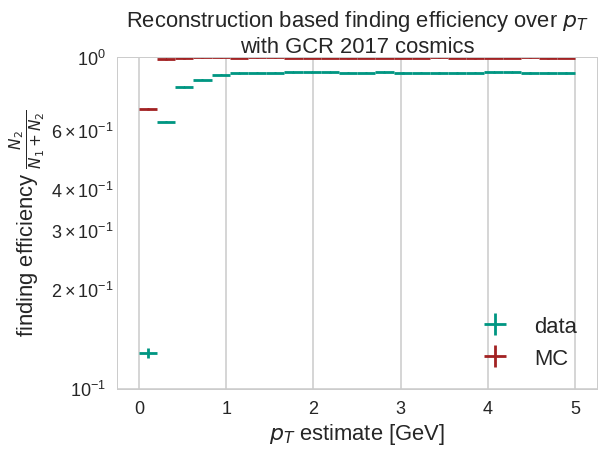
\includegraphics[width=0.46\textwidth]{figures/findeff_pt_data_mc.png}
      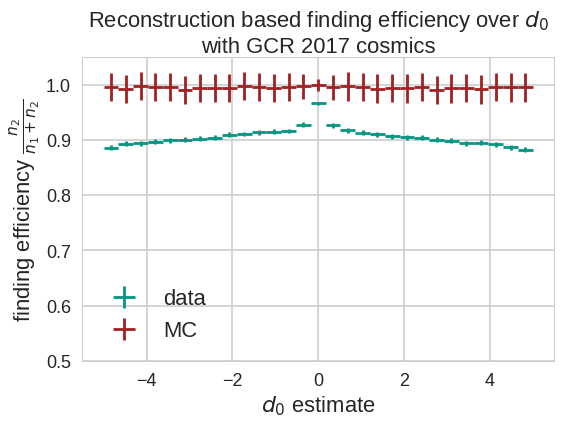
\includegraphics[width=0.46\textwidth]{figures/findeff_d0_data_mc.png}
    \end{center}
  \end{frame}
  
  \begin{frame}
    \begin{center}
      \includegraphics[width=0.46\textwidth]{figures/findeff_tan_lambda_data_mc.png}
      \includegraphics[width=0.46\textwidth]{figures/findeff_z0_data_mc.png}\\
      \includegraphics[width=0.46\textwidth]{figures/findeff_phi0_data_mc.png}
    \end{center}
  \end{frame}
  
  \backupend
  
\end{document}

%%% Local Variables:
%%% ispell-local-dictionary: "en_GB-large_hunspell"
%%% mode: latex
%%% TeX-master: t
%%% End: